\documentclass[conf]{new-aiaa}
%\documentclass[journal]{new-aiaa} %for journal papers
%\documentclass[a4paper]{article}
%\documentclass{homework}

%% Sets page size and margins
%\usepackage[a4paper,top=3cm,bottom=2cm,left=3cm,right=3cm,marginparwidth=0.8.75cm]{geometry}

%\usepackage[utf8]{inputenc}
\usepackage{graphicx}
\usepackage{amsmath}
\usepackage[version=4]{mhchem}
\usepackage{siunitx}
\usepackage{longtable,tabularx}
\setlength\LTleft{0pt} 
%======================================

% additions
\graphicspath{ {figures/} }
\usepackage{floatrow}
\usepackage{ar}
\usepackage{amstext} % for \text macro
\usepackage{array}   % for \newcolumntype macro
\usepackage{gensymb} % for degree symbol
\newcolumntype{L}{>{$}l<{$}} % math-mode version of "l" column type
\usepackage[numbered,framed]{matlab-prettifier}

\pagestyle{empty}

\definecolor{listinggray}{gray}{0.9}
\definecolor{lbcolor}{rgb}{0.9,0.9,0.9}
\lstset{
backgroundcolor=\color{lbcolor},
    tabsize=4,    
%   rulecolor=,
    language=fortran,
        basicstyle=\mlttfamily,
        upquote=true,
        aboveskip={1.5\baselineskip},
        columns=fixed,
        showstringspaces=false,
        extendedchars=false,
        breaklines=true,
        prebreak = \raisebox{0ex}[0ex][0ex]{\ensuremath{\hookleftarrow}},
        frame=single,
        numbers=left,
        showtabs=false,
        showspaces=false,
        showstringspaces=false,
        identifierstyle=\mlttfamily,
				keywordstyle=\color{blue}\mlttfamily,
				stringstyle=\color{red}\mlttfamily,
				commentstyle=\color[RGB]{34,139,34}\mlttfamily,
				morecomment=[l][\color{magenta}]{\#}
        %keywordstyle=\color[rgb]{0,0,1},
        %commentstyle=\color[rgb]{0.026,0.112,0.095},
        %stringstyle=\color[rgb]{0.627,0.126,0.941},
        %numberstyle=\color[rgb]{0.205, 0.142, 0.73},
%        \lstdefinestyle{C++}{language=C++,style=numbers}’.
}
%\usepackage{titlesec}
%\titleformat*{\paragraph}{\large\bfseries}
%======================================
\title{CE 791 HPC - Assignment 5\\MPI - 1D GW Flow Equation}

\author{Andrew Navratil}

\begin{document}

\maketitle

The Jacobi code in Fortran was modified to implement the various versions of MPI calls for solving the inhomogeneous groundwater flow problem.  The jacobi.bsub file was modified for the number of processors and used to queue execution on henry2.  The Mflops were written to the fjacobi.out file and manually copied into the Matlab code after each run based on number of processors.  Calculation of Mflops was updated to account for the 8 flops per call using the Jacobi approximation to the inhomogeneous problem.  The Matlab code then produced the plots for Mflops vs. number of processors for each version of the code.  The different MPI calls are included in the same source file, with a variable for version used to switch between them.  The values for k and h were also saved to txt files on a few of the runs and plotted using Matlab to confirm the correct values were being calculated.  Confirmation was performed by comparing to the analytical plots of K-field and Head field from lecture notes. \\

II(ii): The error value was recalculated for the inhomogeneous problem using the analytical formula.  The function f(x) was created Matlab and utilized to calculate f(0) and f(10) in order to plug into the h formula to determine the constants c0 and c1.  The corresponding h formula with constants was then coded into the Fortran program for error calculation, with the average error calculated using the original square root of the sum of the squares procedure.  The resulting error was printed to the screen to help verify the accuracy of the code changes.  Error values for each version were all about $\num{6.88e-5}$. \\

II(iii): The average leakage flux through the entire aquifer is about $-0.05468$.  This was computed on one of the runs using a second order central difference formula for $\frac{dh}{dx}$, and summing the Q values across all the points of the grid.  We note that both h and k have an x dependence, which makes the analytical solution to compare a little tricky, so that work was abandoned.  A first order backwards difference for $\frac{dh}{dx}$ was also tested, giving the same answer for four significant digits.

\begin{align*}
	Q_{total} &= \int_{0}^{10} k A \frac{dh}{dx} dx = \sum_{i=1}^{n} A k(i) 
		\frac{h(i+1) - h(i-1)}{2} dx
\end{align*}

III(i): The communications in version 1 are buffer dependent and could result in a deadlock or no parallel processing.  The sends and receives can be reordered so they are paired to ensure that any process will finish doing a receive before doing it's own send.  This can be done using the algorithm from lecture and Gropp et. al. where sends and receives are paired for even and odd processors, see version 1 (safe). \\

Plots for Mflops versus number of processors are shown below for each version.  Each version after 0 saw an increase in performance with an increase in the number of processors.  The unsafe version 1 seemed to perform the best, followed by version 3, then version 5, then version 4, then version 2.  Version 0 decreased in performance with increasing number of processors after 1.

\begin{figure}[H]
	\centering
	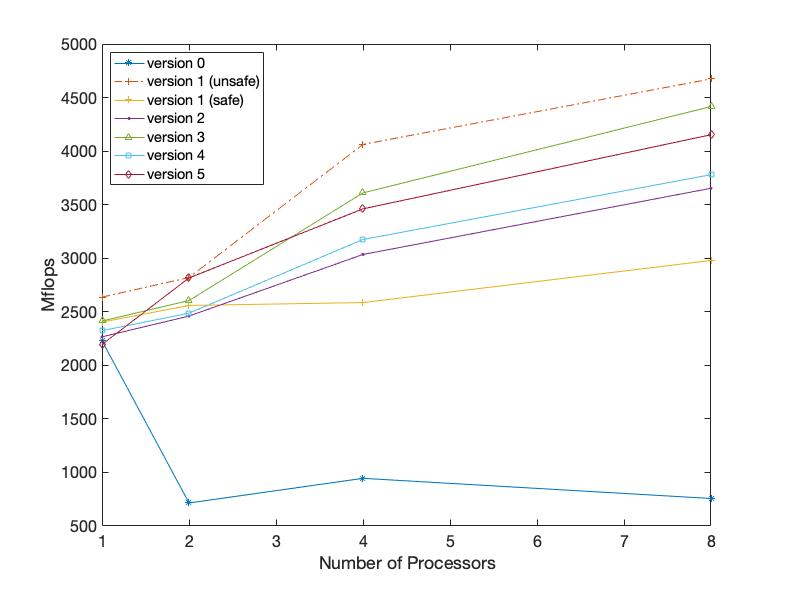
\includegraphics[width=1\columnwidth]{../hw5data/mflops.jpg}
	\caption{version comparison on Mflops}
\end{figure}

%======================================
\newpage
\section*{Fortran Code: Jacobi}
\lstinputlisting[language=fortran]{../a5/jacobi.f90}

\newpage

\section*{Matlab Code}

\lstset{
  style      = Matlab-editor,
  basicstyle = \mlttfamily,
}
\lstinputlisting{../hw5.m}


\end{document}



